\section{Introduction}

The Rubin Observatory Data Management System, as described in \textit{Juric et al}\cite{2015arXiv151207914J},
is responsible for creating the software, services, and systems that will be used to
produce the observatory's science-ready data products.  Project requirements on DM
products are documented in change-controlled specifications. DM Verification and Validation activities are planned
to guarantee that survey software and infrastructure both fulfill the system requirements and enable the science that
motivates the project.

In line with the verification approach adopted for the Gaia DPAC project, described in in \textit{Comoretto et al}\cite{10.1117/12.926797}, 
we present here the tooling and procedures used at Rubin Observatory for the documentation of verification and
validation activities. Test activities are managed in Jira, where test cases are created and updated, and test results
are reported. This ensures that all elements to be documented are available in one tool, that maintains a history of
the process. The System Engineering model is synced with the Jira test framework, providing a direct link between
tests and requirements. Test documents can therefore be generated programmatically, avoiding typical problems
such as a lack of traceability, misspelling, duplication of content, and misalignment between documents. The
centralized collection of information permits a high level of automation, where the extraction of test documents is
achieved by a continuous integration process. This systematic approach substantially reduces the time required to
produce verification and validation documentation, and its integration with the project's System Engineering model, 
detailed in \textit{Selvy et al}\cite{10.1117/12.2310125}, ensures full traceability to system requirements.


\section{The Verification and Validation Problem}

The main scope of the verification and validation activity is to ensure that all requirements have been properly implemented and verified.
This includes identifying the requirements, the affected components and the verification procedures.

The Data Management requirements are baselined in the \textit{Data Management Requirement Specification}\cite{LSE-61}, also know as DMSR.
The DM requirements are flowed down from the SRD, the \textit{LSST System Science Requirements Document} \cite{LPM-17}. 
Interface requirements between DM and other LSST subsystems also have an impact on Data Management provided components, 
and therefore need to be considered during Verification and Validation. 
The figure \ref{fig:topdoctree} shows the high level requirements documents flow down.

\begin{figure}
\begin{center}
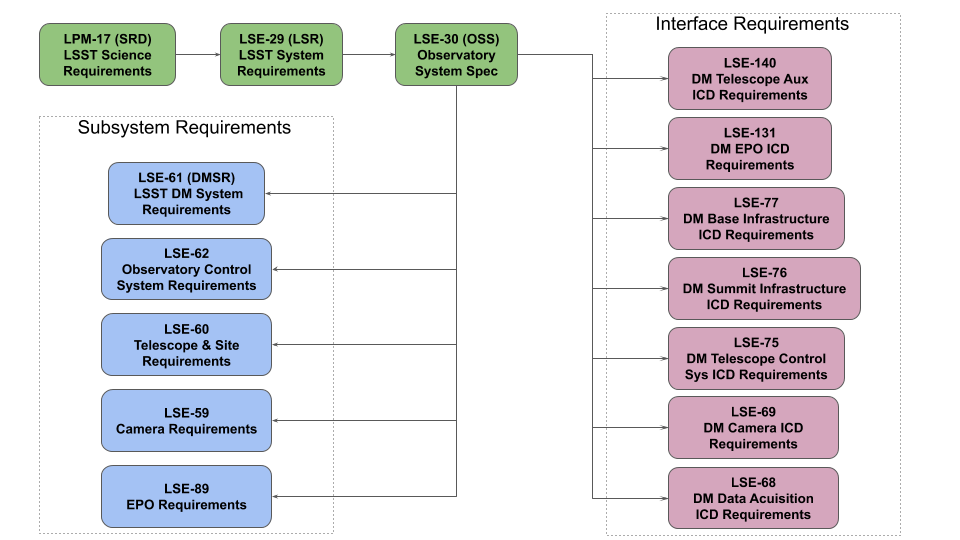
\includegraphics[width=\textwidth]{imgs/TopLevelDocTree.png}
 \caption{The Rubin Observatory top level document tree.}
 \label{fig:topdoctree}
\end{center}
\end{figure}

DM is responsible to fully verify the DMSR requirements and to contribute to the verification and validation of the interface requirements that have an impact on the subsystem.
We guarantee this by creating verification elements associated with each requirement to be verified.
Those verification elements are assigned to the validation scientist, 
who will ensure they are properly described and are sufficient to fully verify the corresponding requirements. 
The validation scientist will ensure also that for each verification element there is at least a test case.
In the case that the provided verification elements are not sufficient, the validation scientist will request more verification elements to be associated with the requirement.
In the opposite case, if a provided verification element is not needed, it will be removed.

The verification and validation activities are organized in test campaigns, each of them is related with milestones, defined at project level.
The results of the test executions are collected in Jira and coverage information is propagated back to Verification Elements and Requirements.
Test documents, including test reports, are generated automatically from Jira.

\begin{figure}
\begin{center}
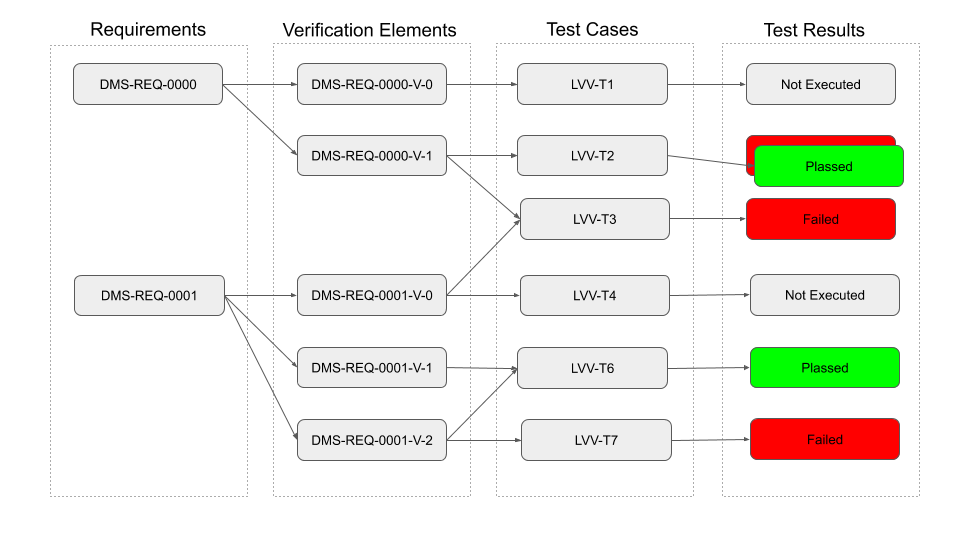
\includegraphics[width=\textwidth]{imgs/VandVSchema.png}
 \caption{Schematic approach to the Verification and Validation.}
 \label{fig:vandvschema}
\end{center}
\end{figure}

The approach ensures that all elements required for the tests are related each other, and are all available in Jira.
This ensures traceability, and makes possible to extract the information in the test documents, without the need of manual intervention.
Figure \ref{fig:vandvschema} shows the relation between each of them.


\section{The Approach}

The verification and validation approach as illustrated in  \textit{Selvy et al}\cite{10.1117/12.2310125}  has been implemented.
Required tools have been put in place, like \textit{Syndeia} and \textit{Docsteady}.
Others tools used in the process described in \ref{sec:proc}, are also generally used in other project activities. 


\subsection{The Tools Used}

Here is given a short description for each tool involved in the Verification and Validation activity.
Figure \ref{fig:vandvtools} gives a schematic overview.

\begin{figure}
\begin{center}
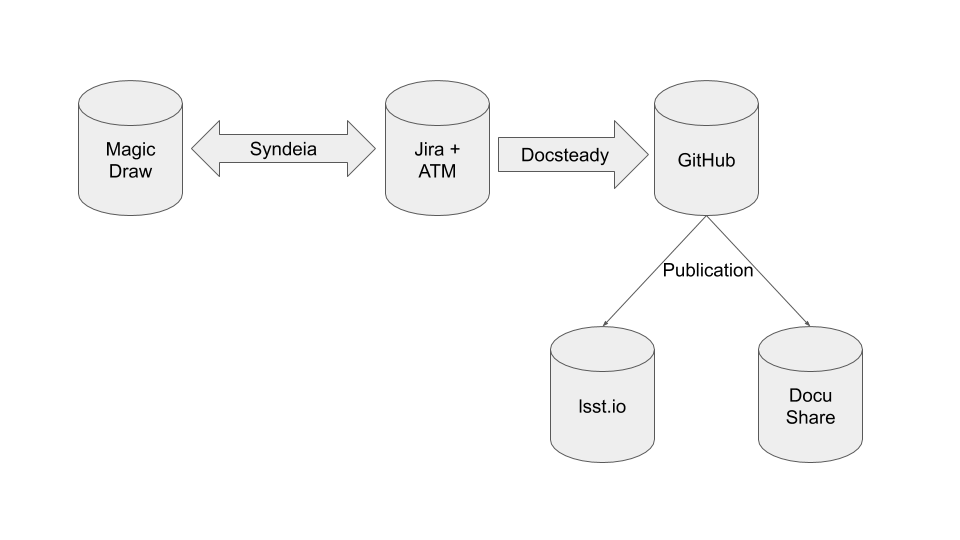
\includegraphics[width=\textwidth]{imgs/VandVtools.png}
 \caption{Schematic overview of the tools involved in the V\&V process.}
 \label{fig:vandvtools}
\end{center}
\end{figure}

\paragraph{MagicDraw}
is the Rubin Observatory Modeling tool. It is used for maintaining the project model and for requirement management. 
The Verification Elements are created in MagicDraw using the requirements as stating point, 
then they are synchronized to and from Jira using \textbf{Syndeia}. 
This ensures that the proper traceability between requirements and verification elements is in place, 
and that changes in one part of the system can be propagated through other components.

\paragraph{Jira}
is the Rubin Observatory issue tracking system.
The Adaptavist Test Manager plugin (ATM) provides additional functionalities to Jira to manage test activities.
Jira is hosting all test information, providing to the user an easy-to-use graphic interface.

\paragraph{Syndeia}
is a third party tool that integrates MagicDraw and Jira. First the Verification Elements created in MagicDraw,
are synched in Jira. After the test activity is completed, the information will be synched back to MagicDraw.

\paragraph{Docsteady}
is the tool that permits generation of the test documents, extracting the information from Jira using REST API.
It can be executed manually or automatically, generating the documents in \LaTeX~format.
It can be scheduled on a continuous integration tool like for example Jenkins, making possible that 
the documents are generated continuously.
The extracted documents are managed using Git repositories, and follows the  DM document workflow.
Docsteady is developed internally in DM and the source code is available at \url{https://github.com/lsst-dm/docsteady}.

\paragraph{GitHub}
is the platform for software version management.
Verification and Validation documents are written in \LaTeX and maintained in Git repositories.
Each time a change is made in the document, a new pdf is built automatically in the integrated Travis platform, and made available in \textbf{lsst.io}.

\paragraph{lsst.io}
is the documentation portal for LSST, see \textit{The LSST the Docs Platform for Continuous Documentation Delivery}\cite{SQR-006}.
Each document has a lsst.io publication page, where the pdf is pushed by Travis, after each successful build.

\paragraph{Docushare}
is the official Rubin Observatory documentation repository during construction.
Documents are uploaded in Docushare only after their formal approval.


\subsection{Process Overview}\label{sec:proc}

The Verification and Validation activities originate from the requirements.
We assume in this document, that the requirements have been properly formalized, documented and approved.
As described early in this paper, a defined number of verification elements is created for each requirement.
When first created, the verification elements have no description. The only information they have is the requirement from where they have been generated.
They are synched to Jira using Syndeia, where the validation scientist ensures that they are properly addressed.
Figure  \ref{fig:vandvtools} gives a graphical overview of the process.

\begin{figure}
\begin{center}
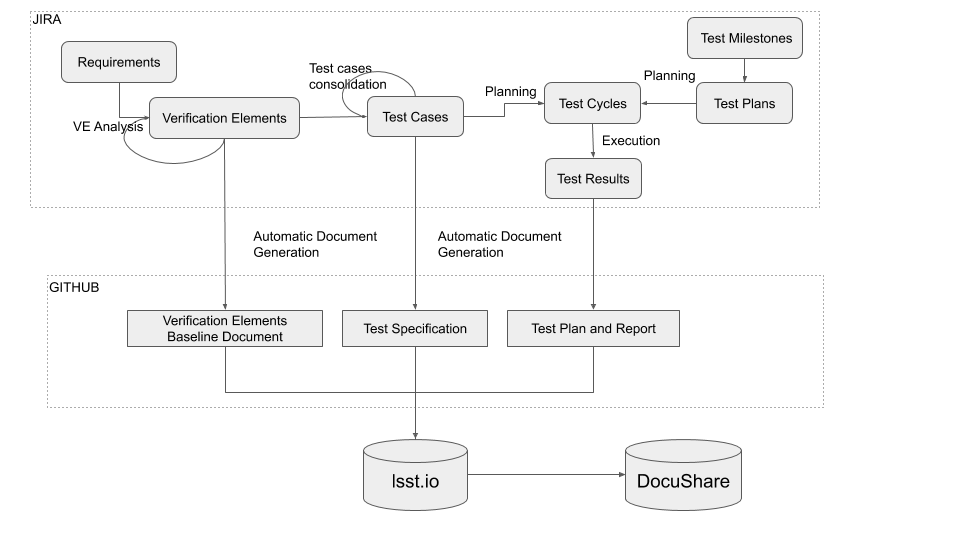
\includegraphics[width=\textwidth]{imgs/VandVprocedure.png}
 \caption{Schematic overview of the V\&V procedure.}
 \label{fig:vandvtools}
\end{center}
\end{figure}

The following subsections describe the main steps of the verification and validation activities that take place in Jira.


\subsubsection{Verification Elements Analysis}

The first activity, required before starting with any test campaign, is to ensure that each verification elements is completed with the relevant information.
This is done by the validation scientist, or delegated.

As a result of the analysis, the verification element will have a description, that describes its scope: which aspect of the requirement will be verified.
Also, the verification element will be related with one or more draft test cases, which are just defined with a one sentence objective and an owner.
Each test case is in this way automatically traced to a verification element and therefore to a requirement.
Verification Elements are baselined in a \textit{Verification Baseline Document}.

\subsubsection{Test Cases Consolidation}

The owner of each test case is in charge to complete it, providing all relevant information. 
This includes also drafting the steps in the detailed test procedure.
Additional test cases can be created, and related to a verification element in order to guarantee the traceability.
In general, test cases can be related with multiple verification elements, and therefore with more than one requirement.

Test cases shall be general, and just specify the software component or the dataset type required. 
However, the exact software or dataset version, or the configuration to be used during the test shall never specified a test case. 
That type of information is provided the test campaign planing phase.
When test cases are instantiated in a test campaign, small adjustments may be done.
Test Cases are baselined in \textit{Test Specifications}.

\subsubsection{Planning and Execution}

As we already mentioned above, the test activities are organized in test campaigns.
For each test campaign, two Jira ATM objects have to be created:

\begin{itemize}
\item \textbf{Jira ATM Test Plan} that provides the context of the test activity, and usually corresponds to a project milestone.
\item \textbf{Jira ATM Test Cycle}(s) that provides the scope. For each test campaign we may have multiple test cycles, 
depending on the different configurations, datasets, or extra conditions we may want to test. Each Test Cycle is traced
to the Jira ATM Test Plan, and provides the list of test cases that need to be executed.
\end{itemize}

For each test campaign we identify two phases:

\paragraph{Planning}
It is the phase when the test campaign is prepared. All relevant information, like for example software version, datasets to use, hardware or configuration, 
is be collected in the Jira ATM Test Plan and Test Cycle(s). 
At the end of this phase we shall be able to say: \textbf{the test is ready to start}.
Despite in the Rubin Observatory there are no formal Test Readiness Review for each test campaign, 
the tooling and procedures in place permit the person who is responsible for the test activity, and relevant stakeholders, to assess and review the collected information. 
This is done by extracting the information into a document, the \textit{Test Plan and Report}, in GitHub, generating the pdf and making it available
in the corresponding lsst.io landing page. Contributors, reviewers and stakeholders can easily access the produced pdf,
check the content of the test plan, and comment, ask for clarification, or request changes using the GitHub
Pull Request (PR) mechanism or the corresponding Jira issue.
When agreement has been reached, the Jira ATM Test Plan status is changed to \textbf{Approved}. The test activity is ready to start.

The outcome of this first phase is an approved \textit{Test Plan and Report} document to be uploaded in Docushare. 
The document at this stage provides the agreed test procedures and all the necessary information required to execute the tests.

\paragraph{Execution}
In this phase, the testers, identified in the previous test plan phase, are in charge to execute the test procedures and 
document the result of each steps in Jira ATM.
The ATM plugin provides a test player view, where for each step in each test case, it is possible to say if it has been executed successfully or not,
specify the result of the step, and relate any Jira issue that has been found during the test execution.

The test result information is extracted extracted and added to the \textit{Test Plan and Report} document.
Once the test execution is completed, an overall assessment shall be provided in the Jira ATM Test Plan.

As done in the previous phase, the document is generated automatically from Jira and provides an easy way to access the test campaign information.
Stakeholders can review the outcome of the test campaign using the same PR mechanism reported above, 
commenting, asking for more information or changes if required, and finally, when consensus is reached, approve the test campaign result.

The Jira ATM test plan status will then be changed to \textbf{Done}.
At the end of the test campaign, the Test Plan and Report is issued and uploaded to Docushare.


\subsection{Test Documents}

These documents identified in the above steps are generated using the \textbf{Docsteady}.
The generation can be done manually, or automatically.
Automation is particularly useful in case we want to see every day the progress of the previous day published in the lsst.io landing page.

The extraction tool ensures homogeneity of information at all levels in the Verification and Validation activities, 
and permits the user sto concentrate only on the relevant test activities, without the need to worry about any documentation aspect.
Follows a summary of the test document:

\begin{itemize}
\item \textbf{Test Specification}: is a document that baselines the test cases. 
A new issue of the document is done each time there is a substantial change in the test cases definition.
\item \textbf{Test Plan and Report}: is a document that includes for a single test campaign, all planning and execution information. 
It  is issued at two times. The first issue corresponds to the consolidation of the planning activity,  
the second to the finalized test campaign containing the results of the test activities.
\item \textbf{Verification Baseline Document}: is a document that provides a snapshot of the verification elements. 
This content is maintained as Jira issues, and is thus easy to change.
Having a snapshot of the verification elements together in a document makes it possible to assess them and keep history.
Approved versions are uploaded in Docushare and used as a reference in other test documents.
\end{itemize}

Test Specifications and Verification Baseline documents are create on specific components, where components are the main products in a subsystem.


\section{The Verification Control Document}

As it has been described in the above sections, all Rubin Observatory test information is managed in Jira. 
This makes it easy to extract the Verification Control Document (VCD), where we summarize the level of coverage for each requirement.

The VCD is a \LaTeX document generated using the document generation tool Docsteady. 
It is managed in a Github repository, as done for the other test documents, built in Travis and published in lsst.io.

Since the number of requirement and verification elements for the Rubin Observatory is very high --
approximately 700 requirements and 1000 verification elements only in DM -- a separate VCD is generated for each subsystem.
In the document there are 2 main sections:

\begin{itemize}
\item \textbf{Summary Information} where a status overview is given. 
This includes the number of requirements and verification elements covered by passed test cases.
Figure \ref{fig:vcdsum} shows an example extracted from the DM VCD.
\item \textbf{Detailed Information} where for each requirement it is shown which are the verification elements and test cases
and the status of the test cases. Links to the test documents are provided, but not descriptive information.
Figure \ref{fig:vcddetail} shows a detail example extracted from the DM VCD.
\end{itemize}

The VCD becomes an important document for management to know the level of verification and validation that has been achieved so far.
At the same time it can be provided to review panels in order to demonstrate that the expected milestones have been met.

\begin{figure}
\begin{center}
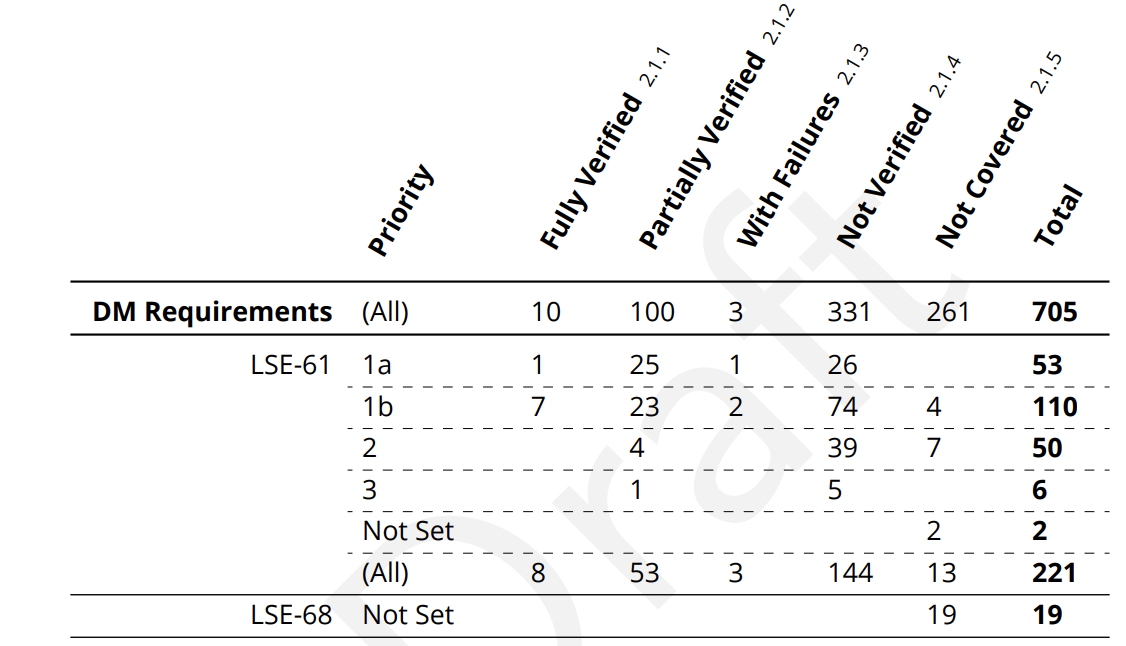
\includegraphics[width=\textwidth]{imgs/VCDsumm.png}
 \caption{Summary example extracted from the DM VCD.}
 \label{fig:vcdsum}
\end{center}
\end{figure}

\begin{figure}
\begin{center}
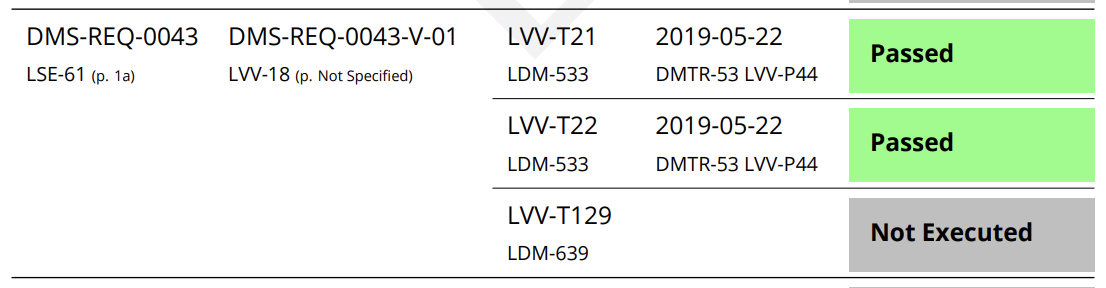
\includegraphics[width=\textwidth]{imgs/VCDdetail.png}
 \caption{Detail example extracted from the DM VCD.}
 \label{fig:vcddetail}
\end{center}
\end{figure}

\section{Conclusions and Outlook}

In the context of a large project like the Rubin Observatory contraction, with a large number of requirements,
some of them very old, the presented approach shows how integrating into the existing infrastructure
custom tools like \textbf{Docsteady} and \textbf{Syndeia}, is possible to see a significant reduction of the effort
required to produce verification and validation documentation.
This permits the team to concentrate on the relevant test activities, maximizing the scientific outcome.

At the same time, automation and continuous integration of the documents generation make test information
much more accessible to the user and stakeholders.
The tooling also ensures that aspects, like traceability between tests and requirements, homogeneity of the information 
or reusability of test cases are easy to implement and provide added value to the process.

Finally, the verification control document provides a global overview of all DM requirements, ensuring we are not forgetting anything.
This approach is not only used by DM, but also by other Rubin Observatory subsystems, that are facing the same challenge.
Using the same tools permit everybody to use the same template and have the same documentation format across the project.



